\documentclass[1p]{elsarticle_modified}
%\bibliographystyle{elsarticle-num}

%\usepackage[colorlinks]{hyperref}
%\usepackage{abbrmath_seonhwa} %\Abb, \Ascr, \Acal ,\Abf, \Afrak
\usepackage{amsfonts}
\usepackage{amssymb}
\usepackage{amsmath}
\usepackage{amsthm}
\usepackage{scalefnt}
\usepackage{amsbsy}
\usepackage{kotex}
\usepackage{caption}
\usepackage{subfig}
\usepackage{color}
\usepackage{graphicx}
\usepackage{xcolor} %% white, black, red, green, blue, cyan, magenta, yellow
\usepackage{float}
\usepackage{setspace}
\usepackage{hyperref}

\usepackage{tikz}
\usetikzlibrary{arrows}

\usepackage{multirow}
\usepackage{array} % fixed length table
\usepackage{hhline}

%%%%%%%%%%%%%%%%%%%%%
\makeatletter
\renewcommand*\env@matrix[1][\arraystretch]{%
	\edef\arraystretch{#1}%
	\hskip -\arraycolsep
	\let\@ifnextchar\new@ifnextchar
	\array{*\c@MaxMatrixCols c}}
\makeatother %https://tex.stackexchange.com/questions/14071/how-can-i-increase-the-line-spacing-in-a-matrix
%%%%%%%%%%%%%%%

\usepackage[normalem]{ulem}

\newcommand{\msout}[1]{\ifmmode\text{\sout{\ensuremath{#1}}}\else\sout{#1}\fi}
%SOURCE: \msout is \stkout macro in https://tex.stackexchange.com/questions/20609/strikeout-in-math-mode

\newcommand{\cancel}[1]{
	\ifmmode
	{\color{red}\msout{#1}}
	\else
	{\color{red}\sout{#1}}
	\fi
}

\newcommand{\add}[1]{
	{\color{blue}\uwave{#1}}
}

\newcommand{\replace}[2]{
	\ifmmode
	{\color{red}\msout{#1}}{\color{blue}\uwave{#2}}
	\else
	{\color{red}\sout{#1}}{\color{blue}\uwave{#2}}
	\fi
}

\newcommand{\Sol}{\mathcal{S}} %segment
\newcommand{\D}{D} %diagram
\newcommand{\A}{\mathcal{A}} %arc


%%%%%%%%%%%%%%%%%%%%%%%%%%%%%5 test

\def\sl{\operatorname{\textup{SL}}(2,\Cbb)}
\def\psl{\operatorname{\textup{PSL}}(2,\Cbb)}
\def\quan{\mkern 1mu \triangleright \mkern 1mu}

\theoremstyle{definition}
\newtheorem{thm}{Theorem}[section]
\newtheorem{prop}[thm]{Proposition}
\newtheorem{lem}[thm]{Lemma}
\newtheorem{ques}[thm]{Question}
\newtheorem{cor}[thm]{Corollary}
\newtheorem{defn}[thm]{Definition}
\newtheorem{exam}[thm]{Example}
\newtheorem{rmk}[thm]{Remark}
\newtheorem{alg}[thm]{Algorithm}

\newcommand{\I}{\sqrt{-1}}
\begin{document}

%\begin{frontmatter}
%
%\title{Boundary parabolic representations of knots up to 8 crossings}
%
%%% Group authors per affiliation:
%\author{Yunhi Cho} 
%\address{Department of Mathematics, University of Seoul, Seoul, Korea}
%\ead{yhcho@uos.ac.kr}
%
%
%\author{Seonhwa Kim} %\fnref{s_kim}}
%\address{Center for Geometry and Physics, Institute for Basic Science, Pohang, 37673, Korea}
%\ead{ryeona17@ibs.re.kr}
%
%\author{Hyuk Kim}
%\address{Department of Mathematical Sciences, Seoul National University, Seoul 08826, Korea}
%\ead{hyukkim@snu.ac.kr}
%
%\author{Seokbeom Yoon}
%\address{Department of Mathematical Sciences, Seoul National University, Seoul, 08826,  Korea}
%\ead{sbyoon15@snu.ac.kr}
%
%\begin{abstract}
%We find all boundary parabolic representation of knots up to 8 crossings.
%
%\end{abstract}
%\begin{keyword}
%    \MSC[2010] 57M25 
%\end{keyword}
%
%\end{frontmatter}

%\linenumbers
%\tableofcontents
%
\newcommand\colored[1]{\textcolor{white}{\rule[-0.35ex]{0.8em}{1.4ex}}\kern-0.8em\color{red} #1}%
%\newcommand\colored[1]{\textcolor{white}{ #1}\kern-2.17ex	\textcolor{white}{ #1}\kern-1.81ex	\textcolor{white}{ #1}\kern-2.15ex\color{red}#1	}

{\Large $\underline{12a_{0050}~(K12a_{0050})}$}

\setlength{\tabcolsep}{10pt}
\renewcommand{\arraystretch}{1.6}
\vspace{1cm}\begin{tabular}{m{100pt}>{\centering\arraybackslash}m{274pt}}
\multirow{5}{120pt}{
	\centering
	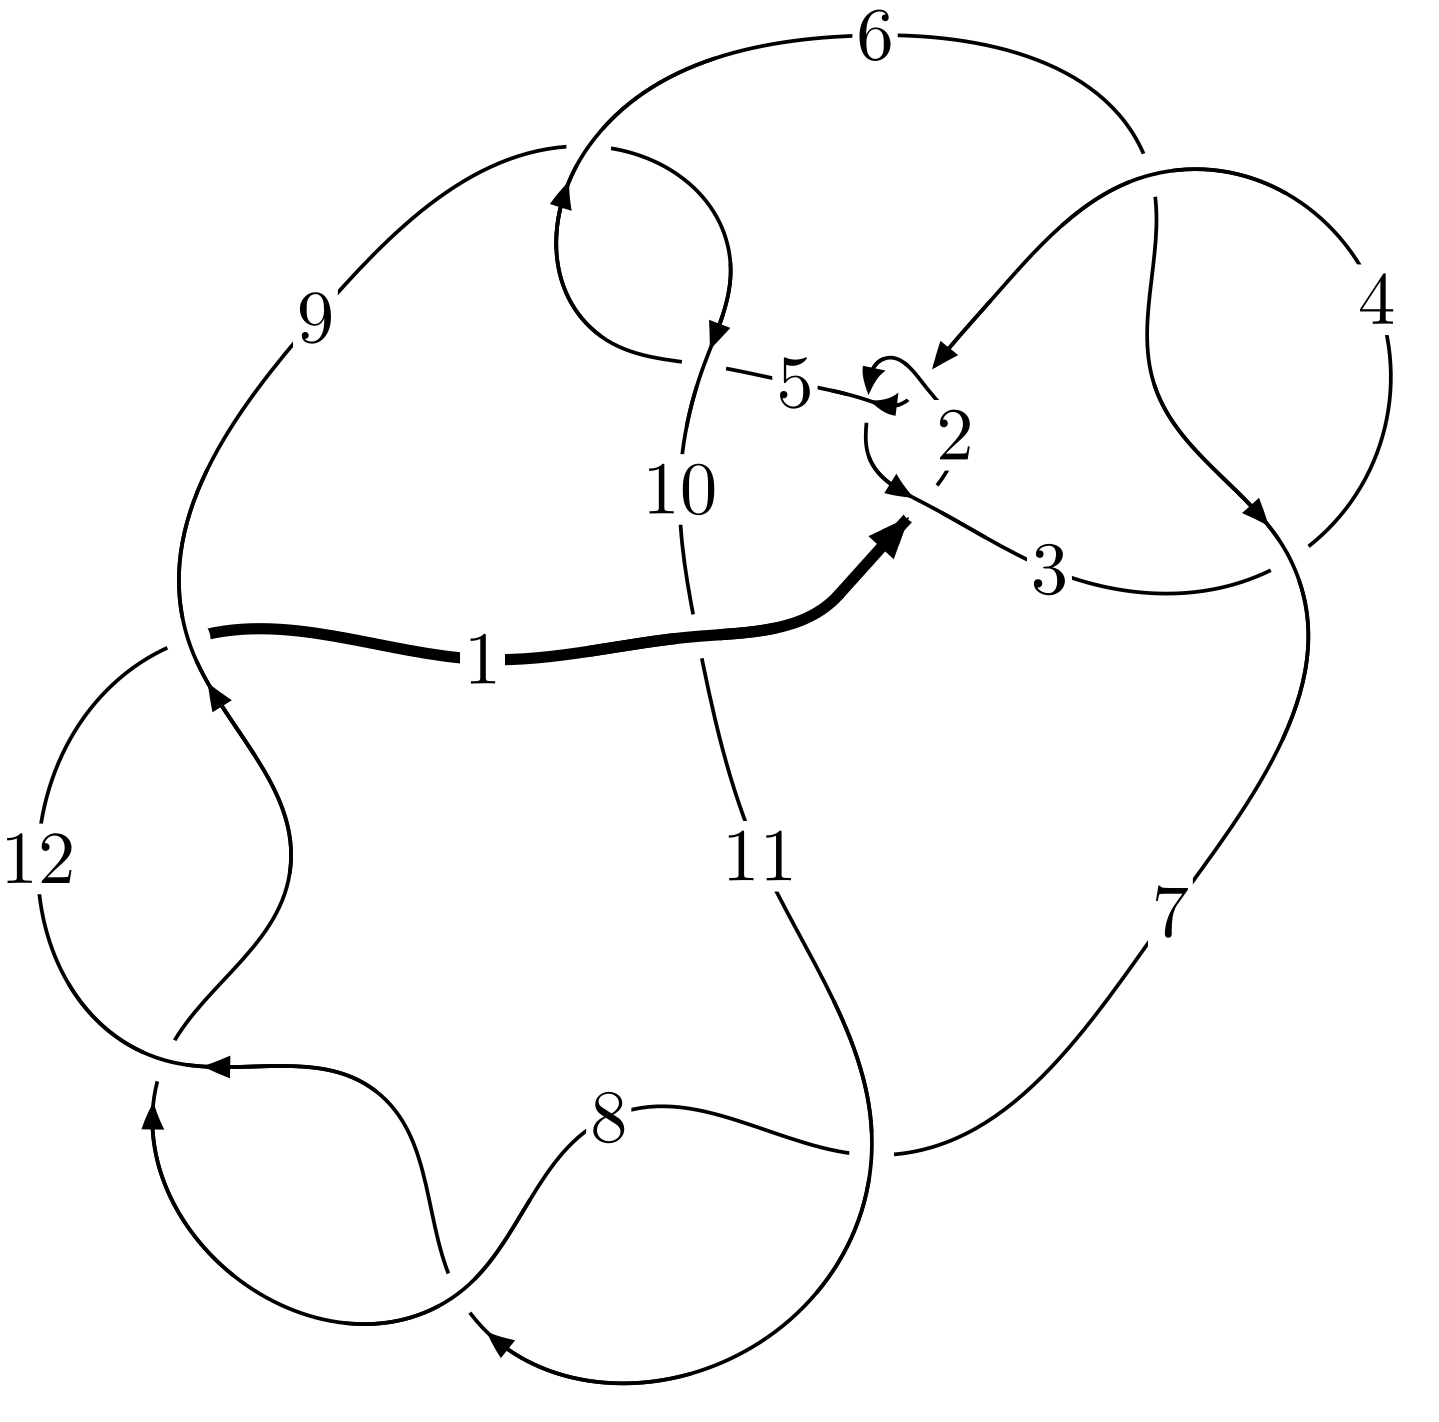
\includegraphics[width=112pt]{../../../GIT/diagram.site/Diagrams/png/851_12a_0050.png}\\
\ \ \ A knot diagram\footnotemark}&
\allowdisplaybreaks
\textbf{Linearized knot diagam} \\
\cline{2-2}
 &
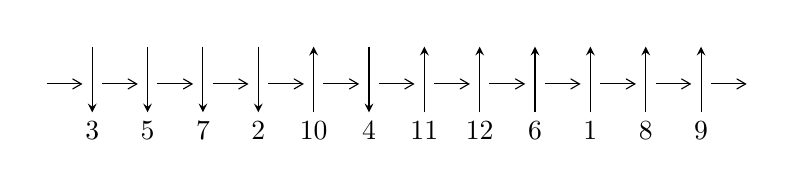
\begin{tikzpicture}[x=20pt, y=17pt]
	% nodes
	\node (C0) at (0, 0) {};
	\node (C1) at (1, 0) {};
	\node (C1U) at (1, +1) {};
	\node (C1D) at (1, -1) {3};

	\node (C2) at (2, 0) {};
	\node (C2U) at (2, +1) {};
	\node (C2D) at (2, -1) {5};

	\node (C3) at (3, 0) {};
	\node (C3U) at (3, +1) {};
	\node (C3D) at (3, -1) {7};

	\node (C4) at (4, 0) {};
	\node (C4U) at (4, +1) {};
	\node (C4D) at (4, -1) {2};

	\node (C5) at (5, 0) {};
	\node (C5U) at (5, +1) {};
	\node (C5D) at (5, -1) {10};

	\node (C6) at (6, 0) {};
	\node (C6U) at (6, +1) {};
	\node (C6D) at (6, -1) {4};

	\node (C7) at (7, 0) {};
	\node (C7U) at (7, +1) {};
	\node (C7D) at (7, -1) {11};

	\node (C8) at (8, 0) {};
	\node (C8U) at (8, +1) {};
	\node (C8D) at (8, -1) {12};

	\node (C9) at (9, 0) {};
	\node (C9U) at (9, +1) {};
	\node (C9D) at (9, -1) {6};

	\node (C10) at (10, 0) {};
	\node (C10U) at (10, +1) {};
	\node (C10D) at (10, -1) {1};

	\node (C11) at (11, 0) {};
	\node (C11U) at (11, +1) {};
	\node (C11D) at (11, -1) {8};

	\node (C12) at (12, 0) {};
	\node (C12U) at (12, +1) {};
	\node (C12D) at (12, -1) {9};
	\node (C13) at (13, 0) {};

	% arrows
	\draw[->,>={angle 60}]
	(C0) edge (C1) (C1) edge (C2) (C2) edge (C3) (C3) edge (C4) (C4) edge (C5) (C5) edge (C6) (C6) edge (C7) (C7) edge (C8) (C8) edge (C9) (C9) edge (C10) (C10) edge (C11) (C11) edge (C12) (C12) edge (C13) ;	\draw[->,>=stealth]
	(C1U) edge (C1D) (C2U) edge (C2D) (C3U) edge (C3D) (C4U) edge (C4D) (C5D) edge (C5U) (C6U) edge (C6D) (C7D) edge (C7U) (C8D) edge (C8U) (C9D) edge (C9U) (C10D) edge (C10U) (C11D) edge (C11U) (C12D) edge (C12U) ;
	\end{tikzpicture} \\
\hhline{~~} \\& 
\textbf{Solving Sequence} \\ \cline{2-2} 
 &
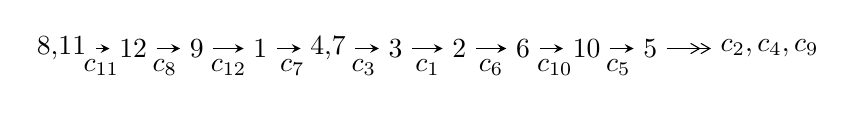
\begin{tikzpicture}[x=23pt, y=7pt]
	% node
	\node (A0) at (-1/8, 0) {8,11};
	\node (A1) at (1, 0) {12};
	\node (A2) at (2, 0) {9};
	\node (A3) at (3, 0) {1};
	\node (A4) at (65/16, 0) {4,7};
	\node (A5) at (41/8, 0) {3};
	\node (A6) at (49/8, 0) {2};
	\node (A7) at (57/8, 0) {6};
	\node (A8) at (65/8, 0) {10};
	\node (A9) at (73/8, 0) {5};
	\node (C1) at (1/2, -1) {$c_{11}$};
	\node (C2) at (3/2, -1) {$c_{8}$};
	\node (C3) at (5/2, -1) {$c_{12}$};
	\node (C4) at (7/2, -1) {$c_{7}$};
	\node (C5) at (37/8, -1) {$c_{3}$};
	\node (C6) at (45/8, -1) {$c_{1}$};
	\node (C7) at (53/8, -1) {$c_{6}$};
	\node (C8) at (61/8, -1) {$c_{10}$};
	\node (C9) at (69/8, -1) {$c_{5}$};
	\node (A10) at (11, 0) {$c_{2},c_{4},c_{9}$};

	% edge
	\draw[->,>=stealth]	
	(A0) edge (A1) (A1) edge (A2) (A2) edge (A3) (A3) edge (A4) (A4) edge (A5) (A5) edge (A6) (A6) edge (A7) (A7) edge (A8) (A8) edge (A9) ;
	\draw[->>,>={angle 60}]	
	(A9) edge (A10);
\end{tikzpicture} \\ 

\end{tabular} \\

\footnotetext{
The image of knot diagram is generated by the software ``\textbf{Draw programme}" developed by Andrew Bartholomew(\url{http://www.layer8.co.uk/maths/draw/index.htm\#Running-draw}), where we modified some parts for our purpose(\url{https://github.com/CATsTAILs/LinksPainter}).
}\phantom \\ \newline 
\centering \textbf{Ideals for irreducible components\footnotemark of $X_{\text{par}}$} 
 
\begin{align*}
I^u_{1}&=\langle 
2.41187\times10^{28} u^{86}-8.03613\times10^{28} u^{85}+\cdots+8.45678\times10^{26} b-1.28690\times10^{28},\\
\phantom{I^u_{1}}&\phantom{= \langle  }-1.57728\times10^{28} u^{86}+4.79845\times10^{28} u^{85}+\cdots+1.26852\times10^{27} a-9.45453\times10^{26},\\
\phantom{I^u_{1}}&\phantom{= \langle  }u^{87}-5 u^{86}+\cdots-12 u+1\rangle \\
I^u_{2}&=\langle 
- u^5+u^4+3 u^3- u^2+b-2 u-2,\;u^5- u^4-3 u^3+u^2+a+2 u+2,\;u^6- u^5-3 u^4+2 u^3+2 u^2+u-1\rangle \\
I^u_{3}&=\langle 
5 a^2 u+9 a^2-17 a u+11 b-13 a+3 u+12,\;a^3-2 a^2 u- a^2-2 a u+3 a-7 u+3,\;u^2+u-1\rangle \\
\\
\end{align*}
\raggedright * 3 irreducible components of $\dim_{\mathbb{C}}=0$, with total 99 representations.\\
\footnotetext{All coefficients of polynomials are rational numbers. But the coefficients are sometimes approximated in decimal forms when there is not enough margin.}
\newpage
\renewcommand{\arraystretch}{1}
\centering \section*{I. $I^u_{1}= \langle 2.41\times10^{28} u^{86}-8.04\times10^{28} u^{85}+\cdots+8.46\times10^{26} b-1.29\times10^{28},\;-1.58\times10^{28} u^{86}+4.80\times10^{28} u^{85}+\cdots+1.27\times10^{27} a-9.45\times10^{26},\;u^{87}-5 u^{86}+\cdots-12 u+1 \rangle$}
\flushleft \textbf{(i) Arc colorings}\\
\begin{tabular}{m{7pt} m{180pt} m{7pt} m{180pt} }
\flushright $a_{8}=$&$\begin{pmatrix}0\\u\end{pmatrix}$ \\
\flushright $a_{11}=$&$\begin{pmatrix}1\\0\end{pmatrix}$ \\
\flushright $a_{12}=$&$\begin{pmatrix}1\\- u^2\end{pmatrix}$ \\
\flushright $a_{9}=$&$\begin{pmatrix}u\\- u^3+u\end{pmatrix}$ \\
\flushright $a_{1}=$&$\begin{pmatrix}- u^2+1\\u^4-2 u^2\end{pmatrix}$ \\
\flushright $a_{4}=$&$\begin{pmatrix}12.4341 u^{86}-37.8273 u^{85}+\cdots+73.4069 u+0.745322\\-28.5200 u^{86}+95.0259 u^{85}+\cdots-184.859 u+15.2174\end{pmatrix}$ \\
\flushright $a_{7}=$&$\begin{pmatrix}- u\\u\end{pmatrix}$ \\
\flushright $a_{3}=$&$\begin{pmatrix}-23.4679 u^{86}+86.4564 u^{85}+\cdots-189.281 u+23.9765\\7.38192 u^{86}-29.2577 u^{85}+\cdots+77.8285 u-8.01379\end{pmatrix}$ \\
\flushright $a_{2}=$&$\begin{pmatrix}-12.9963 u^{86}+40.5794 u^{85}+\cdots-77.7307 u+2.64155\\23.6604 u^{86}-78.3808 u^{85}+\cdots+153.528 u-12.6789\end{pmatrix}$ \\
\flushright $a_{6}=$&$\begin{pmatrix}35.4668 u^{86}-123.526 u^{85}+\cdots+266.381 u-20.1274\\-44.3507 u^{86}+155.563 u^{85}+\cdots-328.649 u+28.6288\end{pmatrix}$ \\
\flushright $a_{10}=$&$\begin{pmatrix}- u^6+3 u^4-2 u^2+1\\u^8-4 u^6+4 u^4\end{pmatrix}$ \\
\flushright $a_{5}=$&$\begin{pmatrix}-12.8929 u^{86}+44.8571 u^{85}+\cdots-91.9941 u+11.8160\\2.22886 u^{86}-7.05574 u^{85}+\cdots+16.1967 u-1.77867\end{pmatrix}$\\&\end{tabular}
\flushleft \textbf{(ii) Obstruction class $= -1$}\\~\\
\flushleft \textbf{(iii) Cusp Shapes $= -\frac{10273217624408414786374874349}{422838840952911474609384418} u^{86}+\frac{33680189062042541632794753137}{422838840952911474609384418} u^{85}+\cdots-\frac{52187858752987512639204783279}{422838840952911474609384418} u-\frac{411818702336231626307587519}{422838840952911474609384418}$}\\~\\
\newpage\renewcommand{\arraystretch}{1}
\flushleft \textbf{(iv) u-Polynomials at the component}\newline \\
\begin{tabular}{m{50pt}|m{274pt}}
Crossings & \hspace{64pt}u-Polynomials at each crossing \\
\hline $$\begin{aligned}c_{1}\end{aligned}$$&$\begin{aligned}
&u^{87}+41 u^{86}+\cdots+1968 u+1
\end{aligned}$\\
\hline $$\begin{aligned}c_{2},c_{4}\end{aligned}$$&$\begin{aligned}
&u^{87}-9 u^{86}+\cdots+42 u+1
\end{aligned}$\\
\hline $$\begin{aligned}c_{3},c_{6}\end{aligned}$$&$\begin{aligned}
&u^{87}-3 u^{86}+\cdots-512 u+64
\end{aligned}$\\
\hline $$\begin{aligned}c_{5},c_{9}\end{aligned}$$&$\begin{aligned}
&u^{87}-2 u^{86}+\cdots-224 u-64
\end{aligned}$\\
\hline $$\begin{aligned}c_{7},c_{8},c_{11}\\c_{12}\end{aligned}$$&$\begin{aligned}
&u^{87}-5 u^{86}+\cdots-12 u+1
\end{aligned}$\\
\hline $$\begin{aligned}c_{10}\end{aligned}$$&$\begin{aligned}
&u^{87}+23 u^{86}+\cdots-19872 u+337
\end{aligned}$\\
\hline
\end{tabular}\\~\\
\newpage\renewcommand{\arraystretch}{1}
\flushleft \textbf{(v) Riley Polynomials at the component}\newline \\
\begin{tabular}{m{50pt}|m{274pt}}
Crossings & \hspace{64pt}Riley Polynomials at each crossing \\
\hline $$\begin{aligned}c_{1}\end{aligned}$$&$\begin{aligned}
&y^{87}+19 y^{86}+\cdots+3775568 y-1
\end{aligned}$\\
\hline $$\begin{aligned}c_{2},c_{4}\end{aligned}$$&$\begin{aligned}
&y^{87}-41 y^{86}+\cdots+1968 y-1
\end{aligned}$\\
\hline $$\begin{aligned}c_{3},c_{6}\end{aligned}$$&$\begin{aligned}
&y^{87}+45 y^{86}+\cdots+139264 y-4096
\end{aligned}$\\
\hline $$\begin{aligned}c_{5},c_{9}\end{aligned}$$&$\begin{aligned}
&y^{87}+40 y^{86}+\cdots+29696 y-4096
\end{aligned}$\\
\hline $$\begin{aligned}c_{7},c_{8},c_{11}\\c_{12}\end{aligned}$$&$\begin{aligned}
&y^{87}-101 y^{86}+\cdots+152 y-1
\end{aligned}$\\
\hline $$\begin{aligned}c_{10}\end{aligned}$$&$\begin{aligned}
&y^{87}-5 y^{86}+\cdots+506574140 y-113569
\end{aligned}$\\
\hline
\end{tabular}\\~\\
\newpage\flushleft \textbf{(vi) Complex Volumes and Cusp Shapes}
$$\begin{array}{c|c|c}  
\text{Solutions to }I^u_{1}& \I (\text{vol} + \sqrt{-1}CS) & \text{Cusp shape}\\
 \hline 
\begin{aligned}
u &= \phantom{-}1.010010 + 0.280355 I \\
a &= -0.454171 + 0.318801 I \\
b &= -0.363009 - 1.195620 I\end{aligned}
 & \phantom{-}1.86315 - 5.76624 I & \phantom{-0.000000 } 0 \\ \hline\begin{aligned}
u &= \phantom{-}1.010010 - 0.280355 I \\
a &= -0.454171 - 0.318801 I \\
b &= -0.363009 + 1.195620 I\end{aligned}
 & \phantom{-}1.86315 + 5.76624 I & \phantom{-0.000000 } 0 \\ \hline\begin{aligned}
u &= \phantom{-}0.891141 + 0.294012 I \\
a &= \phantom{-}0.201900 - 0.412796 I \\
b &= \phantom{-}0.47945 + 1.39754 I\end{aligned}
 & \phantom{-}3.78271 - 0.75026 I & \phantom{-0.000000 } 0 \\ \hline\begin{aligned}
u &= \phantom{-}0.891141 - 0.294012 I \\
a &= \phantom{-}0.201900 + 0.412796 I \\
b &= \phantom{-}0.47945 - 1.39754 I\end{aligned}
 & \phantom{-}3.78271 + 0.75026 I & \phantom{-0.000000 } 0 \\ \hline\begin{aligned}
u &= -0.728506 + 0.562808 I \\
a &= -0.003687 - 0.438604 I \\
b &= -0.18441 + 1.95219 I\end{aligned}
 & -0.38906 - 13.27690 I & \phantom{-0.000000 } 0 \\ \hline\begin{aligned}
u &= -0.728506 - 0.562808 I \\
a &= -0.003687 + 0.438604 I \\
b &= -0.18441 - 1.95219 I\end{aligned}
 & -0.38906 + 13.27690 I & \phantom{-0.000000 } 0 \\ \hline\begin{aligned}
u &= -0.721882 + 0.517254 I \\
a &= \phantom{-}0.181711 + 0.389685 I \\
b &= \phantom{-}0.11772 - 1.87759 I\end{aligned}
 & \phantom{-}2.10446 - 7.61105 I & \phantom{-0.000000 } 0 \\ \hline\begin{aligned}
u &= -0.721882 - 0.517254 I \\
a &= \phantom{-}0.181711 - 0.389685 I \\
b &= \phantom{-}0.11772 + 1.87759 I\end{aligned}
 & \phantom{-}2.10446 + 7.61105 I & \phantom{-0.000000 } 0 \\ \hline\begin{aligned}
u &= -0.672458 + 0.516598 I \\
a &= \phantom{-}0.817277 - 0.015309 I \\
b &= \phantom{-}0.536901 + 0.326251 I\end{aligned}
 & -2.69044 - 6.81997 I & \phantom{-0.000000 } 0 \\ \hline\begin{aligned}
u &= -0.672458 - 0.516598 I \\
a &= \phantom{-}0.817277 + 0.015309 I \\
b &= \phantom{-}0.536901 - 0.326251 I\end{aligned}
 & -2.69044 + 6.81997 I & \phantom{-0.000000 } 0\\
 \hline 
 \end{array}$$\newpage$$\begin{array}{c|c|c}  
\text{Solutions to }I^u_{1}& \I (\text{vol} + \sqrt{-1}CS) & \text{Cusp shape}\\
 \hline 
\begin{aligned}
u &= \phantom{-}0.829810 + 0.126652 I \\
a &= -0.864661 - 0.893648 I \\
b &= \phantom{-}0.09823 + 1.44423 I\end{aligned}
 & -0.281846 - 0.813988 I & \phantom{-0.000000 } 0 \\ \hline\begin{aligned}
u &= \phantom{-}0.829810 - 0.126652 I \\
a &= -0.864661 + 0.893648 I \\
b &= \phantom{-}0.09823 - 1.44423 I\end{aligned}
 & -0.281846 + 0.813988 I & \phantom{-0.000000 } 0 \\ \hline\begin{aligned}
u &= -0.551676 + 0.628089 I \\
a &= \phantom{-}0.446283 - 0.209888 I \\
b &= \phantom{-}0.462139 - 0.044862 I\end{aligned}
 & -4.48506 - 0.94573 I & \phantom{-0.000000 } 0 \\ \hline\begin{aligned}
u &= -0.551676 - 0.628089 I \\
a &= \phantom{-}0.446283 + 0.209888 I \\
b &= \phantom{-}0.462139 + 0.044862 I\end{aligned}
 & -4.48506 + 0.94573 I & \phantom{-0.000000 } 0 \\ \hline\begin{aligned}
u &= -0.633849 + 0.504234 I \\
a &= -0.510764 - 0.726611 I \\
b &= \phantom{-}0.13756 + 1.96218 I\end{aligned}
 & -3.58375 - 4.13631 I & \phantom{-0.000000 } 0 \\ \hline\begin{aligned}
u &= -0.633849 - 0.504234 I \\
a &= -0.510764 + 0.726611 I \\
b &= \phantom{-}0.13756 - 1.96218 I\end{aligned}
 & -3.58375 + 4.13631 I & \phantom{-0.000000 } 0 \\ \hline\begin{aligned}
u &= \phantom{-}0.686979 + 0.423204 I \\
a &= -0.381993 - 0.202436 I \\
b &= \phantom{-}0.78804 + 1.56982 I\end{aligned}
 & \phantom{-}3.84596 + 1.80001 I & \phantom{-0.000000 } 0 \\ \hline\begin{aligned}
u &= \phantom{-}0.686979 - 0.423204 I \\
a &= -0.381993 + 0.202436 I \\
b &= \phantom{-}0.78804 - 1.56982 I\end{aligned}
 & \phantom{-}3.84596 - 1.80001 I & \phantom{-0.000000 } 0 \\ \hline\begin{aligned}
u &= \phantom{-}0.627329 + 0.490479 I \\
a &= \phantom{-}0.496057 + 0.013424 I \\
b &= -0.83681 - 1.57447 I\end{aligned}
 & \phantom{-}2.05491 + 6.93244 I & \phantom{-0.000000 } 0 \\ \hline\begin{aligned}
u &= \phantom{-}0.627329 - 0.490479 I \\
a &= \phantom{-}0.496057 - 0.013424 I \\
b &= -0.83681 + 1.57447 I\end{aligned}
 & \phantom{-}2.05491 - 6.93244 I & \phantom{-0.000000 } 0\\
 \hline 
 \end{array}$$\newpage$$\begin{array}{c|c|c}  
\text{Solutions to }I^u_{1}& \I (\text{vol} + \sqrt{-1}CS) & \text{Cusp shape}\\
 \hline 
\begin{aligned}
u &= -0.415376 + 0.656442 I \\
a &= -0.247896 + 0.519613 I \\
b &= -0.296944 + 0.491125 I\end{aligned}
 & -4.88363 - 3.37848 I & \phantom{-0.000000 } 0 \\ \hline\begin{aligned}
u &= -0.415376 - 0.656442 I \\
a &= -0.247896 - 0.519613 I \\
b &= -0.296944 - 0.491125 I\end{aligned}
 & -4.88363 + 3.37848 I & \phantom{-0.000000 } 0 \\ \hline\begin{aligned}
u &= -0.599038 + 0.447390 I \\
a &= -0.782862 - 0.244572 I \\
b &= -0.414912 - 0.371063 I\end{aligned}
 & -1.18861 - 2.16669 I & \phantom{-0.000000 } 0 \\ \hline\begin{aligned}
u &= -0.599038 - 0.447390 I \\
a &= -0.782862 + 0.244572 I \\
b &= -0.414912 + 0.371063 I\end{aligned}
 & -1.18861 + 2.16669 I & \phantom{-0.000000 } 0 \\ \hline\begin{aligned}
u &= -0.676449 + 0.299656 I \\
a &= \phantom{-}0.756567 - 0.237800 I \\
b &= \phantom{-}0.00819 - 1.44854 I\end{aligned}
 & \phantom{-}4.62680 - 3.56560 I & \phantom{-}7.27157 + 9.65744 I \\ \hline\begin{aligned}
u &= -0.676449 - 0.299656 I \\
a &= \phantom{-}0.756567 + 0.237800 I \\
b &= \phantom{-}0.00819 + 1.44854 I\end{aligned}
 & \phantom{-}4.62680 + 3.56560 I & \phantom{-}7.27157 - 9.65744 I \\ \hline\begin{aligned}
u &= -0.190684 + 0.682767 I \\
a &= \phantom{-}1.84849 + 0.10243 I \\
b &= -0.022296 + 0.386971 I\end{aligned}
 & -1.98497 + 9.09309 I & \phantom{-0.000000 } 0. - 5.78619 I \\ \hline\begin{aligned}
u &= -0.190684 - 0.682767 I \\
a &= \phantom{-}1.84849 - 0.10243 I \\
b &= -0.022296 - 0.386971 I\end{aligned}
 & -1.98497 - 9.09309 I & \phantom{-0.000000 -}0. + 5.78619 I \\ \hline\begin{aligned}
u &= \phantom{-}0.595986 + 0.335404 I \\
a &= \phantom{-}1.15247 + 0.88242 I \\
b &= \phantom{-}0.095803 - 1.019010 I\end{aligned}
 & -0.41312 + 1.89802 I & \phantom{-}2.53218 - 5.30507 I \\ \hline\begin{aligned}
u &= \phantom{-}0.595986 - 0.335404 I \\
a &= \phantom{-}1.15247 - 0.88242 I \\
b &= \phantom{-}0.095803 + 1.019010 I\end{aligned}
 & -0.41312 - 1.89802 I & \phantom{-}2.53218 + 5.30507 I\\
 \hline 
 \end{array}$$\newpage$$\begin{array}{c|c|c}  
\text{Solutions to }I^u_{1}& \I (\text{vol} + \sqrt{-1}CS) & \text{Cusp shape}\\
 \hline 
\begin{aligned}
u &= -0.159142 + 0.620290 I \\
a &= -1.93738 - 0.18215 I \\
b &= \phantom{-}0.042132 - 0.161742 I\end{aligned}
 & \phantom{-}0.45494 + 3.75851 I & \phantom{-}2.39831 - 2.27831 I \\ \hline\begin{aligned}
u &= -0.159142 - 0.620290 I \\
a &= -1.93738 + 0.18215 I \\
b &= \phantom{-}0.042132 + 0.161742 I\end{aligned}
 & \phantom{-}0.45494 - 3.75851 I & \phantom{-}2.39831 + 2.27831 I \\ \hline\begin{aligned}
u &= -0.598200 + 0.200921 I \\
a &= -1.088720 + 0.625520 I \\
b &= -0.056104 + 1.282070 I\end{aligned}
 & \phantom{-}4.04708 + 2.36658 I & \phantom{-}3.70340 + 8.40480 I \\ \hline\begin{aligned}
u &= -0.598200 - 0.200921 I \\
a &= -1.088720 - 0.625520 I \\
b &= -0.056104 - 1.282070 I\end{aligned}
 & \phantom{-}4.04708 - 2.36658 I & \phantom{-}3.70340 - 8.40480 I \\ \hline\begin{aligned}
u &= -0.229873 + 0.585003 I \\
a &= -0.237608 + 0.897450 I \\
b &= \phantom{-}0.011505 + 0.833562 I\end{aligned}
 & -3.98249 + 3.05201 I & -2.80405 - 2.05356 I \\ \hline\begin{aligned}
u &= -0.229873 - 0.585003 I \\
a &= -0.237608 - 0.897450 I \\
b &= \phantom{-}0.011505 - 0.833562 I\end{aligned}
 & -3.98249 - 3.05201 I & -2.80405 + 2.05356 I \\ \hline\begin{aligned}
u &= -0.282835 + 0.551663 I \\
a &= \phantom{-}2.12272 + 0.04738 I \\
b &= -0.537227 + 0.031704 I\end{aligned}
 & -4.60787 + 0.49284 I & -2.55335 - 0.71964 I \\ \hline\begin{aligned}
u &= -0.282835 - 0.551663 I \\
a &= \phantom{-}2.12272 - 0.04738 I \\
b &= -0.537227 - 0.031704 I\end{aligned}
 & -4.60787 - 0.49284 I & -2.55335 + 0.71964 I \\ \hline\begin{aligned}
u &= \phantom{-}0.292776 + 0.514297 I \\
a &= \phantom{-}1.56985 + 0.81715 I \\
b &= \phantom{-}0.391728 - 0.558737 I\end{aligned}
 & \phantom{-}1.08055 - 3.42442 I & \phantom{-}2.38420 + 1.79720 I \\ \hline\begin{aligned}
u &= \phantom{-}0.292776 - 0.514297 I \\
a &= \phantom{-}1.56985 - 0.81715 I \\
b &= \phantom{-}0.391728 + 0.558737 I\end{aligned}
 & \phantom{-}1.08055 + 3.42442 I & \phantom{-}2.38420 - 1.79720 I\\
 \hline 
 \end{array}$$\newpage$$\begin{array}{c|c|c}  
\text{Solutions to }I^u_{1}& \I (\text{vol} + \sqrt{-1}CS) & \text{Cusp shape}\\
 \hline 
\begin{aligned}
u &= -0.350737 + 0.463289 I \\
a &= -0.205369 - 0.866134 I \\
b &= -0.160390 - 0.592063 I\end{aligned}
 & -1.92348 - 1.04705 I & -0.41462 + 4.62441 I \\ \hline\begin{aligned}
u &= -0.350737 - 0.463289 I \\
a &= -0.205369 + 0.866134 I \\
b &= -0.160390 + 0.592063 I\end{aligned}
 & -1.92348 + 1.04705 I & -0.41462 - 4.62441 I \\ \hline\begin{aligned}
u &= \phantom{-}1.41295 + 0.17256 I \\
a &= -0.516333 - 0.548345 I \\
b &= \phantom{-}0.201492 + 1.207130 I\end{aligned}
 & \phantom{-}0.95643 + 6.36363 I & \phantom{-0.000000 } 0 \\ \hline\begin{aligned}
u &= \phantom{-}1.41295 - 0.17256 I \\
a &= -0.516333 + 0.548345 I \\
b &= \phantom{-}0.201492 - 1.207130 I\end{aligned}
 & \phantom{-}0.95643 - 6.36363 I & \phantom{-0.000000 } 0 \\ \hline\begin{aligned}
u &= \phantom{-}1.42426 + 0.02648 I \\
a &= -0.79902 + 1.28037 I \\
b &= \phantom{-}0.25311 - 1.81147 I\end{aligned}
 & \phantom{-}0.53938 + 1.34945 I & \phantom{-0.000000 } 0 \\ \hline\begin{aligned}
u &= \phantom{-}1.42426 - 0.02648 I \\
a &= -0.79902 - 1.28037 I \\
b &= \phantom{-}0.25311 + 1.81147 I\end{aligned}
 & \phantom{-}0.53938 - 1.34945 I & \phantom{-0.000000 } 0 \\ \hline\begin{aligned}
u &= -1.46571 + 0.05632 I \\
a &= -0.051547 + 0.571568 I \\
b &= -0.189919 + 0.027666 I\end{aligned}
 & \phantom{-}6.64268 + 1.76311 I & \phantom{-0.000000 } 0 \\ \hline\begin{aligned}
u &= -1.46571 - 0.05632 I \\
a &= -0.051547 - 0.571568 I \\
b &= -0.189919 - 0.027666 I\end{aligned}
 & \phantom{-}6.64268 - 1.76311 I & \phantom{-0.000000 } 0 \\ \hline\begin{aligned}
u &= \phantom{-}1.47372 + 0.06877 I \\
a &= \phantom{-}0.188121 + 0.967063 I \\
b &= \phantom{-}0.32808 - 1.44311 I\end{aligned}
 & \phantom{-}4.00953 + 2.73511 I & \phantom{-0.000000 } 0 \\ \hline\begin{aligned}
u &= \phantom{-}1.47372 - 0.06877 I \\
a &= \phantom{-}0.188121 - 0.967063 I \\
b &= \phantom{-}0.32808 + 1.44311 I\end{aligned}
 & \phantom{-}4.00953 - 2.73511 I & \phantom{-0.000000 } 0\\
 \hline 
 \end{array}$$\newpage$$\begin{array}{c|c|c}  
\text{Solutions to }I^u_{1}& \I (\text{vol} + \sqrt{-1}CS) & \text{Cusp shape}\\
 \hline 
\begin{aligned}
u &= \phantom{-}0.487248 + 0.192015 I \\
a &= \phantom{-}1.60102 + 0.93973 I \\
b &= -1.32640 - 1.87157 I\end{aligned}
 & -1.041640 + 0.182607 I & \phantom{-}4.12606 - 13.21729 I \\ \hline\begin{aligned}
u &= \phantom{-}0.487248 - 0.192015 I \\
a &= \phantom{-}1.60102 - 0.93973 I \\
b &= -1.32640 + 1.87157 I\end{aligned}
 & -1.041640 - 0.182607 I & \phantom{-}4.12606 + 13.21729 I \\ \hline\begin{aligned}
u &= \phantom{-}0.509388\phantom{ +0.000000I} \\
a &= -0.679237\phantom{ +0.000000I} \\
b &= \phantom{-}0.383628\phantom{ +0.000000I}\end{aligned}
 & \phantom{-}0.764590\phantom{ +0.000000I} & \phantom{-}13.1770\phantom{ +0.000000I} \\ \hline\begin{aligned}
u &= \phantom{-}0.131672 + 0.482233 I \\
a &= -1.86437 - 0.77008 I \\
b &= -0.267014 + 0.371744 I\end{aligned}
 & \phantom{-}2.25594 + 1.34746 I & \phantom{-}3.93001 - 3.94443 I \\ \hline\begin{aligned}
u &= \phantom{-}0.131672 - 0.482233 I \\
a &= -1.86437 + 0.77008 I \\
b &= -0.267014 - 0.371744 I\end{aligned}
 & \phantom{-}2.25594 - 1.34746 I & \phantom{-}3.93001 + 3.94443 I \\ \hline\begin{aligned}
u &= \phantom{-}1.52856 + 0.19143 I \\
a &= \phantom{-}0.408104 + 0.063979 I \\
b &= -0.616967 - 0.460387 I\end{aligned}
 & \phantom{-}2.36054 + 3.92288 I & \phantom{-0.000000 } 0 \\ \hline\begin{aligned}
u &= \phantom{-}1.52856 - 0.19143 I \\
a &= \phantom{-}0.408104 - 0.063979 I \\
b &= -0.616967 + 0.460387 I\end{aligned}
 & \phantom{-}2.36054 - 3.92288 I & \phantom{-0.000000 } 0 \\ \hline\begin{aligned}
u &= -1.57166 + 0.06729 I \\
a &= -2.08529 + 3.23114 I \\
b &= \phantom{-}1.90322 - 3.71902 I\end{aligned}
 & \phantom{-}6.18518 - 1.19455 I & \phantom{-0.000000 } 0 \\ \hline\begin{aligned}
u &= -1.57166 - 0.06729 I \\
a &= -2.08529 - 3.23114 I \\
b &= \phantom{-}1.90322 + 3.71902 I\end{aligned}
 & \phantom{-}6.18518 + 1.19455 I & \phantom{-0.000000 } 0 \\ \hline\begin{aligned}
u &= \phantom{-}1.57641 + 0.12488 I \\
a &= -0.571783 + 0.472057 I \\
b &= \phantom{-}1.289790 - 0.459669 I\end{aligned}
 & \phantom{-}6.19157 + 4.23438 I & \phantom{-0.000000 } 0\\
 \hline 
 \end{array}$$\newpage$$\begin{array}{c|c|c}  
\text{Solutions to }I^u_{1}& \I (\text{vol} + \sqrt{-1}CS) & \text{Cusp shape}\\
 \hline 
\begin{aligned}
u &= \phantom{-}1.57641 - 0.12488 I \\
a &= -0.571783 - 0.472057 I \\
b &= \phantom{-}1.289790 + 0.459669 I\end{aligned}
 & \phantom{-}6.19157 - 4.23438 I & \phantom{-0.000000 } 0 \\ \hline\begin{aligned}
u &= -1.57932 + 0.09454 I \\
a &= -0.247972 + 0.844562 I \\
b &= -0.362527 - 0.626041 I\end{aligned}
 & \phantom{-}7.02868 - 3.46437 I & \phantom{-0.000000 } 0 \\ \hline\begin{aligned}
u &= -1.57932 - 0.09454 I \\
a &= -0.247972 - 0.844562 I \\
b &= -0.362527 + 0.626041 I\end{aligned}
 & \phantom{-}7.02868 + 3.46437 I & \phantom{-0.000000 } 0 \\ \hline\begin{aligned}
u &= \phantom{-}1.58242 + 0.06903 I \\
a &= -0.29201 - 2.76631 I \\
b &= \phantom{-}0.57137 + 3.68365 I\end{aligned}
 & \phantom{-}11.55840 - 1.29646 I & \phantom{-0.000000 } 0 \\ \hline\begin{aligned}
u &= \phantom{-}1.58242 - 0.06903 I \\
a &= -0.29201 + 2.76631 I \\
b &= \phantom{-}0.57137 - 3.68365 I\end{aligned}
 & \phantom{-}11.55840 + 1.29646 I & \phantom{-0.000000 } 0 \\ \hline\begin{aligned}
u &= -1.58519\phantom{ +0.000000I} \\
a &= \phantom{-}0.997201\phantom{ +0.000000I} \\
b &= -0.668948\phantom{ +0.000000I}\end{aligned}
 & \phantom{-}8.07273\phantom{ +0.000000I} & \phantom{-0.000000 } 0 \\ \hline\begin{aligned}
u &= -1.58073 + 0.14082 I \\
a &= -1.78005 + 2.09338 I \\
b &= \phantom{-}1.45293 - 2.87581 I\end{aligned}
 & \phantom{-}9.51389 - 9.24025 I & \phantom{-0.000000 } 0 \\ \hline\begin{aligned}
u &= -1.58073 - 0.14082 I \\
a &= -1.78005 - 2.09338 I \\
b &= \phantom{-}1.45293 + 2.87581 I\end{aligned}
 & \phantom{-}9.51389 + 9.24025 I & \phantom{-0.000000 } 0 \\ \hline\begin{aligned}
u &= \phantom{-}1.58150 + 0.14435 I \\
a &= -0.90877 - 3.37832 I \\
b &= \phantom{-}0.76910 + 4.06653 I\end{aligned}
 & \phantom{-}3.89012 + 6.50742 I & \phantom{-0.000000 } 0 \\ \hline\begin{aligned}
u &= \phantom{-}1.58150 - 0.14435 I \\
a &= -0.90877 + 3.37832 I \\
b &= \phantom{-}0.76910 - 4.06653 I\end{aligned}
 & \phantom{-}3.89012 - 6.50742 I & \phantom{-0.000000 } 0\\
 \hline 
 \end{array}$$\newpage$$\begin{array}{c|c|c}  
\text{Solutions to }I^u_{1}& \I (\text{vol} + \sqrt{-1}CS) & \text{Cusp shape}\\
 \hline 
\begin{aligned}
u &= \phantom{-}1.59599 + 0.09211 I \\
a &= \phantom{-}0.40709 + 2.92156 I \\
b &= -0.51286 - 3.84759 I\end{aligned}
 & \phantom{-}12.39170 + 5.06306 I & \phantom{-0.000000 } 0 \\ \hline\begin{aligned}
u &= \phantom{-}1.59599 - 0.09211 I \\
a &= \phantom{-}0.40709 - 2.92156 I \\
b &= -0.51286 + 3.84759 I\end{aligned}
 & \phantom{-}12.39170 - 5.06306 I & \phantom{-0.000000 } 0 \\ \hline\begin{aligned}
u &= \phantom{-}1.59413 + 0.15161 I \\
a &= \phantom{-}0.653822 - 0.295842 I \\
b &= -1.396300 + 0.079914 I\end{aligned}
 & \phantom{-}4.96648 + 9.29592 I & \phantom{-0.000000 } 0 \\ \hline\begin{aligned}
u &= \phantom{-}1.59413 - 0.15161 I \\
a &= \phantom{-}0.653822 + 0.295842 I \\
b &= -1.396300 - 0.079914 I\end{aligned}
 & \phantom{-}4.96648 - 9.29592 I & \phantom{-0.000000 } 0 \\ \hline\begin{aligned}
u &= -1.59938 + 0.11914 I \\
a &= \phantom{-}1.61226 - 2.32414 I \\
b &= -1.40674 + 3.07633 I\end{aligned}
 & \phantom{-}11.62610 - 3.80327 I & \phantom{-0.000000 } 0 \\ \hline\begin{aligned}
u &= -1.59938 - 0.11914 I \\
a &= \phantom{-}1.61226 + 2.32414 I \\
b &= -1.40674 - 3.07633 I\end{aligned}
 & \phantom{-}11.62610 + 3.80327 I & \phantom{-0.000000 } 0 \\ \hline\begin{aligned}
u &= -1.61679 + 0.03544 I \\
a &= \phantom{-}0.83922 - 1.17901 I \\
b &= -0.380596 + 1.248080 I\end{aligned}
 & \phantom{-}8.04740 + 0.17742 I & \phantom{-0.000000 } 0 \\ \hline\begin{aligned}
u &= -1.61679 - 0.03544 I \\
a &= \phantom{-}0.83922 + 1.17901 I \\
b &= -0.380596 - 1.248080 I\end{aligned}
 & \phantom{-}8.04740 - 0.17742 I & \phantom{-0.000000 } 0 \\ \hline\begin{aligned}
u &= \phantom{-}1.61192 + 0.15359 I \\
a &= \phantom{-}0.97184 + 2.89964 I \\
b &= -0.70154 - 3.73677 I\end{aligned}
 & \phantom{-}10.0164 + 10.1316 I & \phantom{-0.000000 } 0 \\ \hline\begin{aligned}
u &= \phantom{-}1.61192 - 0.15359 I \\
a &= \phantom{-}0.97184 - 2.89964 I \\
b &= -0.70154 + 3.73677 I\end{aligned}
 & \phantom{-}10.0164 - 10.1316 I & \phantom{-0.000000 } 0\\
 \hline 
 \end{array}$$\newpage$$\begin{array}{c|c|c}  
\text{Solutions to }I^u_{1}& \I (\text{vol} + \sqrt{-1}CS) & \text{Cusp shape}\\
 \hline 
\begin{aligned}
u &= \phantom{-}1.61482 + 0.17017 I \\
a &= -1.12043 - 2.77461 I \\
b &= \phantom{-}0.75341 + 3.59107 I\end{aligned}
 & \phantom{-}7.5322 + 16.0397 I & \phantom{-0.000000 } 0 \\ \hline\begin{aligned}
u &= \phantom{-}1.61482 - 0.17017 I \\
a &= -1.12043 + 2.77461 I \\
b &= \phantom{-}0.75341 - 3.59107 I\end{aligned}
 & \phantom{-}7.5322 - 16.0397 I & \phantom{-0.000000 } 0 \\ \hline\begin{aligned}
u &= -1.65448 + 0.06893 I \\
a &= \phantom{-}0.76967 - 2.45752 I \\
b &= -0.91725 + 3.16651 I\end{aligned}
 & \phantom{-}12.58290 - 0.59134 I & \phantom{-0.000000 } 0 \\ \hline\begin{aligned}
u &= -1.65448 - 0.06893 I \\
a &= \phantom{-}0.76967 + 2.45752 I \\
b &= -0.91725 - 3.16651 I\end{aligned}
 & \phantom{-}12.58290 + 0.59134 I & \phantom{-0.000000 } 0 \\ \hline\begin{aligned}
u &= -1.67615 + 0.04835 I \\
a &= -0.48336 + 2.26752 I \\
b &= \phantom{-}0.78811 - 2.96006 I\end{aligned}
 & \phantom{-}11.19340 + 4.66031 I & \phantom{-0.000000 } 0 \\ \hline\begin{aligned}
u &= -1.67615 - 0.04835 I \\
a &= -0.48336 - 2.26752 I \\
b &= \phantom{-}0.78811 + 2.96006 I\end{aligned}
 & \phantom{-}11.19340 - 4.66031 I & \phantom{-0.000000 } 0 \\ \hline\begin{aligned}
u &= \phantom{-}0.0864028\phantom{ +0.000000I} \\
a &= \phantom{-}6.46516\phantom{ +0.000000I} \\
b &= -0.774246\phantom{ +0.000000I}\end{aligned}
 & -1.21024\phantom{ +0.000000I} & -9.56520\phantom{ +0.000000I}\\
 \hline 
 \end{array}$$\newpage\newpage\renewcommand{\arraystretch}{1}
\centering \section*{II. $I^u_{2}= \langle - u^5+u^4+3 u^3- u^2+b-2 u-2,\;u^5- u^4-3 u^3+u^2+a+2 u+2,\;u^6- u^5-3 u^4+2 u^3+2 u^2+u-1 \rangle$}
\flushleft \textbf{(i) Arc colorings}\\
\begin{tabular}{m{7pt} m{180pt} m{7pt} m{180pt} }
\flushright $a_{8}=$&$\begin{pmatrix}0\\u\end{pmatrix}$ \\
\flushright $a_{11}=$&$\begin{pmatrix}1\\0\end{pmatrix}$ \\
\flushright $a_{12}=$&$\begin{pmatrix}1\\- u^2\end{pmatrix}$ \\
\flushright $a_{9}=$&$\begin{pmatrix}u\\- u^3+u\end{pmatrix}$ \\
\flushright $a_{1}=$&$\begin{pmatrix}- u^2+1\\u^4-2 u^2\end{pmatrix}$ \\
\flushright $a_{4}=$&$\begin{pmatrix}- u^5+u^4+3 u^3- u^2-2 u-2\\u^5- u^4-3 u^3+u^2+2 u+2\end{pmatrix}$ \\
\flushright $a_{7}=$&$\begin{pmatrix}- u\\u\end{pmatrix}$ \\
\flushright $a_{3}=$&$\begin{pmatrix}- u^5+u^4+3 u^3- u^2-2 u-2\\u^5- u^4-3 u^3+u^2+2 u+2\end{pmatrix}$ \\
\flushright $a_{2}=$&$\begin{pmatrix}- u^5+u^4+3 u^3-2 u^2-2 u-1\\u^5-3 u^3- u^2+2 u+2\end{pmatrix}$ \\
\flushright $a_{6}=$&$\begin{pmatrix}- u\\u\end{pmatrix}$ \\
\flushright $a_{10}=$&$\begin{pmatrix}- u^5+2 u^3+u\\u^5-3 u^3+u\end{pmatrix}$ \\
\flushright $a_{5}=$&$\begin{pmatrix}u^2-1\\- u^4+2 u^2\end{pmatrix}$\\&\end{tabular}
\flushleft \textbf{(ii) Obstruction class $= 1$}\\~\\
\flushleft \textbf{(iii) Cusp Shapes $= 10 u^5-6 u^4-38 u^3+5 u^2+33 u+27$}\\~\\
\newpage\renewcommand{\arraystretch}{1}
\flushleft \textbf{(iv) u-Polynomials at the component}\newline \\
\begin{tabular}{m{50pt}|m{274pt}}
Crossings & \hspace{64pt}u-Polynomials at each crossing \\
\hline $$\begin{aligned}c_{1},c_{2}\end{aligned}$$&$\begin{aligned}
&(u-1)^6
\end{aligned}$\\
\hline $$\begin{aligned}c_{3},c_{6}\end{aligned}$$&$\begin{aligned}
&u^6
\end{aligned}$\\
\hline $$\begin{aligned}c_{4}\end{aligned}$$&$\begin{aligned}
&(u+1)^6
\end{aligned}$\\
\hline $$\begin{aligned}c_{5},c_{10}\end{aligned}$$&$\begin{aligned}
&u^6- u^5+3 u^4-2 u^3+2 u^2- u-1
\end{aligned}$\\
\hline $$\begin{aligned}c_{7},c_{8}\end{aligned}$$&$\begin{aligned}
&u^6+u^5-3 u^4-2 u^3+2 u^2- u-1
\end{aligned}$\\
\hline $$\begin{aligned}c_{9}\end{aligned}$$&$\begin{aligned}
&u^6+u^5+3 u^4+2 u^3+2 u^2+u-1
\end{aligned}$\\
\hline $$\begin{aligned}c_{11},c_{12}\end{aligned}$$&$\begin{aligned}
&u^6- u^5-3 u^4+2 u^3+2 u^2+u-1
\end{aligned}$\\
\hline
\end{tabular}\\~\\
\newpage\renewcommand{\arraystretch}{1}
\flushleft \textbf{(v) Riley Polynomials at the component}\newline \\
\begin{tabular}{m{50pt}|m{274pt}}
Crossings & \hspace{64pt}Riley Polynomials at each crossing \\
\hline $$\begin{aligned}c_{1},c_{2},c_{4}\end{aligned}$$&$\begin{aligned}
&(y-1)^6
\end{aligned}$\\
\hline $$\begin{aligned}c_{3},c_{6}\end{aligned}$$&$\begin{aligned}
&y^6
\end{aligned}$\\
\hline $$\begin{aligned}c_{5},c_{9},c_{10}\end{aligned}$$&$\begin{aligned}
&y^6+5 y^5+9 y^4+4 y^3-6 y^2-5 y+1
\end{aligned}$\\
\hline $$\begin{aligned}c_{7},c_{8},c_{11}\\c_{12}\end{aligned}$$&$\begin{aligned}
&y^6-7 y^5+17 y^4-16 y^3+6 y^2-5 y+1
\end{aligned}$\\
\hline
\end{tabular}\\~\\
\newpage\flushleft \textbf{(vi) Complex Volumes and Cusp Shapes}
$$\begin{array}{c|c|c}  
\text{Solutions to }I^u_{2}& \I (\text{vol} + \sqrt{-1}CS) & \text{Cusp shape}\\
 \hline 
\begin{aligned}
u &= -0.493180 + 0.575288 I \\
a &= -0.228804 + 0.434483 I \\
b &= \phantom{-}0.228804 - 0.434483 I\end{aligned}
 & -4.60518 - 1.97241 I & -0.89950 + 4.53432 I \\ \hline\begin{aligned}
u &= -0.493180 - 0.575288 I \\
a &= -0.228804 - 0.434483 I \\
b &= \phantom{-}0.228804 + 0.434483 I\end{aligned}
 & -4.60518 + 1.97241 I & -0.89950 - 4.53432 I \\ \hline\begin{aligned}
u &= \phantom{-}0.483672\phantom{ +0.000000I} \\
a &= -2.83358\phantom{ +0.000000I} \\
b &= \phantom{-}2.83358\phantom{ +0.000000I}\end{aligned}
 & -0.906083\phantom{ +0.000000I} & \phantom{-}39.7680\phantom{ +0.000000I} \\ \hline\begin{aligned}
u &= \phantom{-}1.52087 + 0.16310 I \\
a &= \phantom{-}0.636388 + 0.565801 I \\
b &= -0.636388 - 0.565801 I\end{aligned}
 & \phantom{-}2.05064 + 4.59213 I & \phantom{-}1.73030 - 5.96315 I \\ \hline\begin{aligned}
u &= \phantom{-}1.52087 - 0.16310 I \\
a &= \phantom{-}0.636388 - 0.565801 I \\
b &= -0.636388 + 0.565801 I\end{aligned}
 & \phantom{-}2.05064 - 4.59213 I & \phantom{-}1.73030 + 5.96315 I \\ \hline\begin{aligned}
u &= -1.53904\phantom{ +0.000000I} \\
a &= \phantom{-}2.01841\phantom{ +0.000000I} \\
b &= -2.01841\phantom{ +0.000000I}\end{aligned}
 & \phantom{-}6.01515\phantom{ +0.000000I} & \phantom{-}6.57090\phantom{ +0.000000I}\\
 \hline 
 \end{array}$$\newpage\newpage\renewcommand{\arraystretch}{1}
\centering \section*{III. $I^u_{3}= \langle 5 a^2 u+9 a^2-17 a u+11 b-13 a+3 u+12,\;a^3-2 a^2 u- a^2-2 a u+3 a-7 u+3,\;u^2+u-1 \rangle$}
\flushleft \textbf{(i) Arc colorings}\\
\begin{tabular}{m{7pt} m{180pt} m{7pt} m{180pt} }
\flushright $a_{8}=$&$\begin{pmatrix}0\\u\end{pmatrix}$ \\
\flushright $a_{11}=$&$\begin{pmatrix}1\\0\end{pmatrix}$ \\
\flushright $a_{12}=$&$\begin{pmatrix}1\\u-1\end{pmatrix}$ \\
\flushright $a_{9}=$&$\begin{pmatrix}u\\- u+1\end{pmatrix}$ \\
\flushright $a_{1}=$&$\begin{pmatrix}u\\- u\end{pmatrix}$ \\
\flushright $a_{4}=$&$\begin{pmatrix}a\\-0.454545 a^{2} u+1.54545 a u+\cdots+1.18182 a-1.09091\end{pmatrix}$ \\
\flushright $a_{7}=$&$\begin{pmatrix}- u\\u\end{pmatrix}$ \\
\flushright $a_{3}=$&$\begin{pmatrix}-0.0909091 a^{2} u+0.909091 a u+\cdots+1.63636 a-0.818182\\-0.363636 a^{2} u+0.636364 a u+\cdots+0.545455 a-0.272727\end{pmatrix}$ \\
\flushright $a_{2}=$&$\begin{pmatrix}0.363636 a^{2} u+0.363636 a u+\cdots+0.454545 a-1.72727\\-2 u\end{pmatrix}$ \\
\flushright $a_{6}=$&$\begin{pmatrix}0.0909091 a^{2} u+0.0909091 a u+\cdots+0.363636 a-1.18182\\0.272727 a^{2} u+0.272727 a u+\cdots+0.0909091 a-0.545455\end{pmatrix}$ \\
\flushright $a_{10}=$&$\begin{pmatrix}u\\- u+1\end{pmatrix}$ \\
\flushright $a_{5}=$&$\begin{pmatrix}0.0909091 a^{2} u+0.0909091 a u+\cdots+0.363636 a-1.18182\\0.272727 a^{2} u+0.272727 a u+\cdots+0.0909091 a-0.545455\end{pmatrix}$\\&\end{tabular}
\flushleft \textbf{(ii) Obstruction class $= 1$}\\~\\
\flushleft \textbf{(iii) Cusp Shapes $= -\frac{20}{11} a^2 u-\frac{58}{11} a^2+\frac{57}{11} a u+\frac{107}{11} a+\frac{10}{11} u-\frac{59}{11}$}\\~\\
\newpage\renewcommand{\arraystretch}{1}
\flushleft \textbf{(iv) u-Polynomials at the component}\newline \\
\begin{tabular}{m{50pt}|m{274pt}}
Crossings & \hspace{64pt}u-Polynomials at each crossing \\
\hline $$\begin{aligned}c_{1},c_{3}\end{aligned}$$&$\begin{aligned}
&(u^3- u^2+2 u-1)^2
\end{aligned}$\\
\hline $$\begin{aligned}c_{2}\end{aligned}$$&$\begin{aligned}
&(u^3+u^2-1)^2
\end{aligned}$\\
\hline $$\begin{aligned}c_{4}\end{aligned}$$&$\begin{aligned}
&(u^3- u^2+1)^2
\end{aligned}$\\
\hline $$\begin{aligned}c_{5},c_{9}\end{aligned}$$&$\begin{aligned}
&u^6
\end{aligned}$\\
\hline $$\begin{aligned}c_{6}\end{aligned}$$&$\begin{aligned}
&(u^3+u^2+2 u+1)^2
\end{aligned}$\\
\hline $$\begin{aligned}c_{7},c_{8},c_{10}\end{aligned}$$&$\begin{aligned}
&(u^2- u-1)^3
\end{aligned}$\\
\hline $$\begin{aligned}c_{11},c_{12}\end{aligned}$$&$\begin{aligned}
&(u^2+u-1)^3
\end{aligned}$\\
\hline
\end{tabular}\\~\\
\newpage\renewcommand{\arraystretch}{1}
\flushleft \textbf{(v) Riley Polynomials at the component}\newline \\
\begin{tabular}{m{50pt}|m{274pt}}
Crossings & \hspace{64pt}Riley Polynomials at each crossing \\
\hline $$\begin{aligned}c_{1},c_{3},c_{6}\end{aligned}$$&$\begin{aligned}
&(y^3+3 y^2+2 y-1)^2
\end{aligned}$\\
\hline $$\begin{aligned}c_{2},c_{4}\end{aligned}$$&$\begin{aligned}
&(y^3- y^2+2 y-1)^2
\end{aligned}$\\
\hline $$\begin{aligned}c_{5},c_{9}\end{aligned}$$&$\begin{aligned}
&y^6
\end{aligned}$\\
\hline $$\begin{aligned}c_{7},c_{8},c_{10}\\c_{11},c_{12}\end{aligned}$$&$\begin{aligned}
&(y^2-3 y+1)^3
\end{aligned}$\\
\hline
\end{tabular}\\~\\
\newpage\flushleft \textbf{(vi) Complex Volumes and Cusp Shapes}
$$\begin{array}{c|c|c}  
\text{Solutions to }I^u_{3}& \I (\text{vol} + \sqrt{-1}CS) & \text{Cusp shape}\\
 \hline 
\begin{aligned}
u &= \phantom{-}0.618034\phantom{ +0.000000I} \\
a &= \phantom{-}0.290827 + 0.846791 I \\
b &= \phantom{-}0.057180 + 1.268210 I\end{aligned}
 & \phantom{-}4.01109 - 2.82812 I & \phantom{-}3.00413 + 7.79836 I \\ \hline\begin{aligned}
u &= \phantom{-}0.618034\phantom{ +0.000000I} \\
a &= \phantom{-}0.290827 - 0.846791 I \\
b &= \phantom{-}0.057180 - 1.268210 I\end{aligned}
 & \phantom{-}4.01109 + 2.82812 I & \phantom{-}3.00413 - 7.79836 I \\ \hline\begin{aligned}
u &= \phantom{-}0.618034\phantom{ +0.000000I} \\
a &= \phantom{-}1.65441\phantom{ +0.000000I} \\
b &= -0.732393\phantom{ +0.000000I}\end{aligned}
 & -0.126494\phantom{ +0.000000I} & -0.918090\phantom{ +0.000000I} \\ \hline\begin{aligned}
u &= -1.61803\phantom{ +0.000000I} \\
a &= -2.26961\phantom{ +0.000000I} \\
b &= \phantom{-}1.91743\phantom{ +0.000000I}\end{aligned}
 & \phantom{-}7.76919\phantom{ +0.000000I} & -21.8890\phantom{ +0.000000I} \\ \hline\begin{aligned}
u &= -1.61803\phantom{ +0.000000I} \\
a &= \phantom{-}0.01677 + 2.51235 I \\
b &= -0.14970 - 3.32021 I\end{aligned}
 & \phantom{-}11.90680 - 2.82812 I & \phantom{-}7.89941 + 3.17745 I \\ \hline\begin{aligned}
u &= -1.61803\phantom{ +0.000000I} \\
a &= \phantom{-}0.01677 - 2.51235 I \\
b &= -0.14970 + 3.32021 I\end{aligned}
 & \phantom{-}11.90680 + 2.82812 I & \phantom{-}7.89941 - 3.17745 I\\
 \hline 
 \end{array}$$\newpage
\newpage\renewcommand{\arraystretch}{1}
\centering \section*{ IV. u-Polynomials}
\begin{tabular}{m{50pt}|m{274pt}}
Crossings & \hspace{64pt}u-Polynomials at each crossing \\
\hline $$\begin{aligned}c_{1}\end{aligned}$$&$\begin{aligned}
&((u-1)^6)(u^3- u^2+2 u-1)^2(u^{87}+41 u^{86}+\cdots+1968 u+1)
\end{aligned}$\\
\hline $$\begin{aligned}c_{2}\end{aligned}$$&$\begin{aligned}
&((u-1)^6)(u^3+u^2-1)^2(u^{87}-9 u^{86}+\cdots+42 u+1)
\end{aligned}$\\
\hline $$\begin{aligned}c_{3}\end{aligned}$$&$\begin{aligned}
&u^6(u^3- u^2+2 u-1)^2(u^{87}-3 u^{86}+\cdots-512 u+64)
\end{aligned}$\\
\hline $$\begin{aligned}c_{4}\end{aligned}$$&$\begin{aligned}
&((u+1)^6)(u^3- u^2+1)^2(u^{87}-9 u^{86}+\cdots+42 u+1)
\end{aligned}$\\
\hline $$\begin{aligned}c_{5}\end{aligned}$$&$\begin{aligned}
&u^6(u^6- u^5+\cdots- u-1)(u^{87}-2 u^{86}+\cdots-224 u-64)
\end{aligned}$\\
\hline $$\begin{aligned}c_{6}\end{aligned}$$&$\begin{aligned}
&u^6(u^3+u^2+2 u+1)^2(u^{87}-3 u^{86}+\cdots-512 u+64)
\end{aligned}$\\
\hline $$\begin{aligned}c_{7},c_{8}\end{aligned}$$&$\begin{aligned}
&(u^2- u-1)^3(u^6+u^5-3 u^4-2 u^3+2 u^2- u-1)\\
&\cdot(u^{87}-5 u^{86}+\cdots-12 u+1)
\end{aligned}$\\
\hline $$\begin{aligned}c_{9}\end{aligned}$$&$\begin{aligned}
&u^6(u^6+u^5+\cdots+u-1)(u^{87}-2 u^{86}+\cdots-224 u-64)
\end{aligned}$\\
\hline $$\begin{aligned}c_{10}\end{aligned}$$&$\begin{aligned}
&(u^2- u-1)^3(u^6- u^5+3 u^4-2 u^3+2 u^2- u-1)\\
&\cdot(u^{87}+23 u^{86}+\cdots-19872 u+337)
\end{aligned}$\\
\hline $$\begin{aligned}c_{11},c_{12}\end{aligned}$$&$\begin{aligned}
&(u^2+u-1)^3(u^6- u^5-3 u^4+2 u^3+2 u^2+u-1)\\
&\cdot(u^{87}-5 u^{86}+\cdots-12 u+1)
\end{aligned}$\\
\hline
\end{tabular}\newpage\renewcommand{\arraystretch}{1}
\centering \section*{ V. Riley Polynomials}
\begin{tabular}{m{50pt}|m{274pt}}
Crossings & \hspace{64pt}Riley Polynomials at each crossing \\
\hline $$\begin{aligned}c_{1}\end{aligned}$$&$\begin{aligned}
&((y-1)^6)(y^3+3 y^2+2 y-1)^2(y^{87}+19 y^{86}+\cdots+3775568 y-1)
\end{aligned}$\\
\hline $$\begin{aligned}c_{2},c_{4}\end{aligned}$$&$\begin{aligned}
&((y-1)^6)(y^3- y^2+2 y-1)^2(y^{87}-41 y^{86}+\cdots+1968 y-1)
\end{aligned}$\\
\hline $$\begin{aligned}c_{3},c_{6}\end{aligned}$$&$\begin{aligned}
&y^6(y^3+3 y^2+2 y-1)^2(y^{87}+45 y^{86}+\cdots+139264 y-4096)
\end{aligned}$\\
\hline $$\begin{aligned}c_{5},c_{9}\end{aligned}$$&$\begin{aligned}
&y^6(y^6+5 y^5+9 y^4+4 y^3-6 y^2-5 y+1)\\
&\cdot(y^{87}+40 y^{86}+\cdots+29696 y-4096)
\end{aligned}$\\
\hline $$\begin{aligned}c_{7},c_{8},c_{11}\\c_{12}\end{aligned}$$&$\begin{aligned}
&(y^2-3 y+1)^3(y^6-7 y^5+17 y^4-16 y^3+6 y^2-5 y+1)\\
&\cdot(y^{87}-101 y^{86}+\cdots+152 y-1)
\end{aligned}$\\
\hline $$\begin{aligned}c_{10}\end{aligned}$$&$\begin{aligned}
&(y^2-3 y+1)^3(y^6+5 y^5+9 y^4+4 y^3-6 y^2-5 y+1)\\
&\cdot(y^{87}-5 y^{86}+\cdots+506574140 y-113569)
\end{aligned}$\\
\hline
\end{tabular}
\vskip 2pc
\end{document}